\title{%
  Brewery Boys \\
  \large Predicting Beer Ratings through Singular Value Decomposition and Collaborative Filtering \\
}
\author{
        Matt McFarland and Theodore Owens
}
\date{\today}


\documentclass[12pt]{article}
\renewcommand{\thesubsection}{(\alph{subsection})}

\usepackage[margin=1.0in]{geometry}
\usepackage{graphicx}
\usepackage{amsmath}
\usepackage{amssymb}
\usepackage{csquotes}
\usepackage{enumerate}
\usepackage{listings}
\usepackage{color}
\usepackage{booktabs}
\renewcommand{\abstractname}{\vspace{-\baselineskip}}
\definecolor{mygray}{rgb}{0.9,0.9,0.9}
\lstset{ %
  backgroundcolor=\color{mygray},
  numbers=left,
  breaklines=true
}

\begin{document}
\maketitle
\begin{abstract}
% TODO
Using a dataset of beer reviews from \textbf{Beer Advocate}, we attempt to predict a reviewer's scoring of an unencountered beer based on tastes expressed through their previous reviews. We use two collaborative filtering approaches to make predictions: \textbf{Singular Value Decomposition} and \textbf{Item-to-Item Collaborative Filtering}.

Our baseline establishes...
We find...

\end{abstract}

% Questions for Matt:

% 1. Does order matter when finding the item residual (mean) and the user residual (mean) for the baseline
% 2. ^ Yes. Need to normalize for beer mean bias first. Then get user offset of beer means deltas.

\section{Preface}
To keep our terminology consistent with existing literature in collaborative filtering, we will take \textit{users} to mean reviewers on Beer Advocate and \textit{items} to mean the beers under review. For a user $i$ and an item $j$, let $y_{ij}$ and $\hat y_{ij}$ give the actual and predicted rating of that user on that item, respectively.

\section{Problem}
We are presented with $\mathbf{X}$, an $m \times n$ matrix of $m$ users and their ratings of $n$ items. This matrix is sparse, as most users have only rated a small subset of items. We have no information about the nature of the users (e.g. age, gender) or the nature of the items. Our problem can be phrased as: \textbf{given a user $i$ and an item $j$ that user $i$ has not rated, predict $\hat y_{ij}$}.

\paragraph{Collaborative Filtering} Given the lack of feature information (categorization of items, demographics of users, etc.), we cannot rely on supervised learning techniques. We thus turn to unsupervised methods and collaborative filtering, in particular. Collaborative Filtering techniques attempt to establish similarities in user preferences for certain items based on observed user-item interactions. Predicted ratings rise when a user favorably rates items similar to the predicted item.

\paragraph{Training} This process first requires establishing which items are similar to each other. Intuitively, if a user rates two items in the same fashion (both poorly or both well), then they are similar. If the user rates them oppositely, they are dissimilar. In our SVD analysis, we establish a set of latent features describing items that are similar in some respect, as determined by user preferences. For Item-Based Collaborative Filtering, we generate a correlation matrix that describes the similarity between all pairings of items.

\paragraph{Prediction} Intuitively, if a user favorably rates item $A$, which is quite similar to an unrated item $B$, we expect the user to favorably rate item $B$. In the prediction stage, we make use of the user's provided ratings to make inferences about an unkown rating. In SVD analysis, we can predict the score of an unreviewed item by finding the product of that user's latent feature vector multiplied by that item's latent feature vector.

\section{Data}
Our dataset contains $1,586,599$ reviews concerning $m = 33,388$ users and $n = 65,680$ items. Each review contains a rating on a scale from $0$ to $5$ by intervals of $\frac{1}{2}$. It also provides user rating along several other metrics (palate, taste, appearance, aroma) as well as some information about the item itself (brewery, style, alcohol by volume).

\begin{figure}[!ht]
\begin{center}
\caption{Sample Ratings}
    \includegraphics[width=.9\textwidth]{"./images/dataset_sample".png}
\end{center}
\end{figure}

We limit our analysis to use the primary rating.

\begin{figure}[!ht]
\begin{center}
\caption{Rating Distribution}
    \includegraphics[width=.5\textwidth]{"./images/rating_hist".png}
\end{center}
\end{figure}

In \textit{Figure 2}, we observe that a majority of the ratings fall into the 3.5, 4, and 4.5 categories.

Not all items receive the same number of reviews, nor do all reviewers rate the same number of items. In \textit{Figure 3}, we find that our dataset is highly skewed, with many items and users possessing quite few reviews.

\begin{figure}[!ht]
\caption{Distributions of Number of Ratings by Item and by User}
\centering
\begin{minipage}{.5\textwidth}
  \centering
  \includegraphics[width=0.95\linewidth]{"./images/item_hist".png}
\end{minipage}%
\begin{minipage}{.5\textwidth}
  \centering
  \includegraphics[width=0.95\linewidth]{"./images/user_hist".png}
\end{minipage}
\end{figure}

Each review contains a rating on a scale from $0$ to $5$ by intervals of $\frac{1}{2}$. It also provides user rating along several other metrics (palate, taste, appearance, aroma) as well as some information about the item itself (brewery, style, alcohol by volume). We limit our analysis to use the primary rating (``overall review'').

\section{Pre-Processing}
The dataset is arranged into a list of ratings, where each rating represents one user's rating of one item. To generate our user-by-item matrix $\mathbf{X}$, we must rearrange these reviews and extract the primary rating.

We additionally remove all users who have not rated at least 5 items and all items that have not received at least 50 ratings. The denser the network of users and items, the better we can establish similarities amongst preferences and items. Removing obscure items and reviewers whose tastes are relatively unknown reduces the noise without hindering prediction quality. This leaves us with approximately $5,000$ items and $13,000$ users, where the resulting matrix is 1.8\% filled.

Additionally, we form a modified user-by-item matrix $\mathbf{\bar X}$, where:

$$ \mathbf{\bar X}_{ij} = \mathbf{X}_{ij} - \mu_{user_i} - \mu_{item_j}$$

We derive the $\mu$ terms in our baseline algorithm. Intuitively, $\mathbf{\bar X}$ represents the residual of a rating that is not explained by the item's average (its ``quality'') and the user's rating tendencies.

\subsection{Summary Statistics}

\begin{table}[ht!]
\centering
\caption{Summary Statistics}
\begin{tabular}{ll}
\hline
Number of Reviews         & 1,586,599 \\
Number of Items           & 65,680    \\
Number of Users           & 33,388    \\
Rating Minimum            & 5.0       \\
Rating Maximum            & 0.0       \\
Rating Mean               & 3.82      \\
Rating Variance           & 0.52      \\
Rating Standard Deviation & 0.72      \\ \hline
\end{tabular}
\end{table}

\section{Methods}
We use three methods to make predictions:

\begin{enumerate}
  \item \textbf{Baseline}: use rating means rather than machine learning approaches to establish a baseline prediction against which we can compare our more advanced approaches.
  \item \textbf{Singular Value Decomposition}: uses feature reduction to expose latent features in the items and user preferences.
  \item \textbf{Item-Based Collaborative Filtering}: uses a correlation matrix comparing all pairs of items and predicts based on ratings of similar items
\end{enumerate}

\section{Error Measurement}
In accordance with the literature standard, we evaluate the performance of our algorithms with the Mean Squared Error (MSE) measurement, defined as follows:

% $$ \mathbf{MAE} = \frac{\sum\limits_{i,j \epsilon S} \mathbf{\|Y_{ij} - \hat{Y}_{iy}\|}}{\sum\limits_{i,j \epsilon S}\mathbf{\|S\|} $$
$$ \mathbf{MSE} = \frac{\sum\limits_{i,j \epsilon S} {\mathbf{\|Y_{ij} - \hat{Y}_{iy}\|}}^2}{\sum\limits_{i,j \epsilon S}{\mathbf{\|S\|}}^2} $$

\section{Baseline}
To evaluate the success of our approaches, we first establish a simplified prediction algorithm. For many datasets, this naive approach yields decent results and can be hard to improve upon.

Our baseline algorithm first calculates a series of means. First, we calculate the residual mean for each item, $\mu_{item}$. This gives a sense of the quality and appeal of the item. \textit{After} subtracting both $\mu_{item}$ (for each item) from $\mathbf{X}$, we calculate the residual mean for each user, $\mu_{user}$. This tells us whether a user is a generous or harsh rater.

We form the predicted rating for user $i$ on item $j$ by calculating:

$$\hat y_{ij} = \mu_{user_i} + \mu_{item_j}$$

Put another way, we predict the item's average and adjust for bias introduced by the user's rating tendency (harsh or easy).

\subsection{Results}

\section{Singular Value Decomposition}
\subsection{Background}
\paragraph{Theoretical Basis} Single Value Decomposition is a form of Principal Component Analysis, which factors a matrix $Y$ into component matrices $U * \Sigma * V^{T}$. Principal Component Analysis alters the basis of $Y$ so that, in the factorized form, the directions of greatest variance are exposed in decreasing order. In our dataset, $Y$ represents the user-item interaction matrix, and when we decompose that matrix to constituent parts $U$ and $V$, we will find the eigenvectors of $Y$ that define the directions of greatest variance. Single Value Decomposition limits the factorization to the $K$ most significant eigenvectors. Because $Y$ is very large, but very sparse, we can simplify the data by factoring to $U$ and $V$. Where $U$ is a $n$ by $k$ matrix where each row represents a latent feature vector for a user, and $V$ is a $d$ by $K$ matrix where each row represents the latent feature vector for an item. These latent feature vectors are meaningful because, given an incomplete $Y$ matrix (where not all user-item interactions are accounted for), we can iteratively train $U$ and $V$ to approximate the data we do have for $Y$. New user-item interactions (ratings) are predicted with $\hat{Y}_{ij} = U_{i}V_{j}^{T}$.

\paragraph{Literature Review} Single Value Decomposition used a technique to simplify a large, sparse user-interaction matrix has been used very successfully before, most famously in the famous Netflix Prize\textsuperscript{\cite{gower}}. Studies on the application of SVD to decompose a matrix has revealed several variants on the basic algorithm to increase the accuracy of the predictions. Such methods include adaptively altering the learning rate, changing the iterative update method, and adding regularization\textsuperscript{\cite{ma}}. Other have also added different normalization constants to the SVD analysis to account for quality and user biases\textsuperscript{\cite{paterek}}. Simon Funk, a famous contestant in the Netflix algorithm further tuned the bias weights based on the number of reviews an item or user had \textbf{cite SF post}. Gower explains that successful Netflix SVD algorithms also incorporated time-based information about the user to increase the prediction's accuracy\textsuperscript{\cite{gower}}. The SVD method has been explored extensively, and we will attempt to replicate some of the most successful methods on our dataset.

\subsection{Algorithm}
The goal of the SVD find a $U$ and $V$ matrix that well approximate $Y$. This is accomplished by minimizing the following difference function $E(U,V)$. In order to prevent overtraining, we also regularize for $U$ and $V$. $U$ and $V$ were updated with stochastic gradient descent until the training error increased. 

$$ [\hat{U}, \hat{V}] = \min{\|Y_{ij} - \hat{Y}_{ij}\|}^2 = \min\limits_{U,V}{\|Y_{ij} - U_i V_j^T\|}^2 + w_U\|U\|^2 + w_V\|V\|^2$$

Because $Y$ is incomplete, we cannot solve for the closed form solution and thus must update $U$ and $V$ iteratively with a gradient descent. ($S$ is the set of observed user-item iteractions, and $I$ is the indicator of seen ratings for $Y$.)

$$ \frac{\partial E}{\partial U_i} = -2 * \sum\limits_{i,j \epsilon S} (Y_{ij} - U_i V_j^T) V_j + w_U U_i$$

\begin{center}
  In compact matrix form, this is $\frac{\partial E}{\partial U} = -2 * I (Y - U V^T) U + w_U U$
\end{center}

$$ \frac{\partial E}{\partial V_j} = -2 * \sum\limits_{i,j \epsilon S} (Y_{ij} - U_i V_j^T) U_i + w_V V_j$$

\begin{center}
  In compact matrix form, this is $\frac{\partial E}{\partial V} = -2 * (I (Y - U V^T))^T V + w_V V$
\end{center}

Where $U$ and $V$ were updated with schotastic gradient descent (where $\mu$ is the learning rate / step size)

$$ U_{i+1} = U - \mu * \frac{\partial E}{\partial U} \\$$

$$ V_{i+1} = V - \mu * \frac{\partial E}{\partial V} \\$$

\subsection{Hyper-Parameter Tuning}
There were four hyper-parameters to tune for the regularized SVD: The learning rate, the regulariations weights for $U$ and $V$, and $K$ which determines the number of eigenvalues taken in $U$ and $V$. Because cross-validate testing among all four hyper parameters would be too time intensive, we opted to select the regularization weights $w_U = 20.0$ and $w_V = 10.0$ which generally extended the training as long as possible. We selected a learning rate varying from $0.5 to .001$ depending which data we were training on. We attempted to use the largest training rate that would not diverge.  

Tried different bias methods...

\subsection{Results}

We were able to realize an MSE of $.3286$ which represented an improvement of $2.1\%$ over the bias baseline predictor (MSE of $.3356$). After centering the dataset on item biases and then centering for each user's bias over the centered item scores, we iteratively trained our SVD algorithm on the residuals. We used the previously found successful weights of $w_U = 20.0$ and $w_V = 10.0$ and the determined best $K = 3$ hyperparameter.

\begin{figure}[!ht]
\begin{center}
\caption{SVD Training Results}
    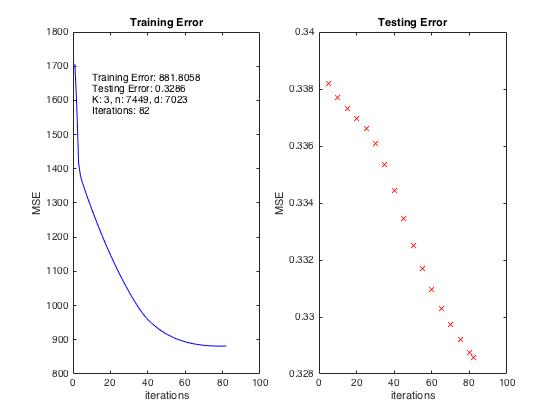
\includegraphics[width=.\textwidth]{./figures/big_full_convergence.jpg}
\end{center}
\end{figure}

\begin{center}
Reviews included: $1,225,865$
Test percentage: $15\%$
N = $7,749$
d = $7,023$
Sparcity = $2.3\%$

\section{Item-Based Collaborative Filtering}

\subsection{Algorithm}
\paragraph{Training} For this method, we similarly begin from our residual feature matrix $\mathbf{\bar X}$. We generate an $n \times n$ correlation matrix $\mathbf{C}$. The entry $\mathbf{C}_{ij}$ describes the similarity of ratings between items $i$ and $j$. If a particular user reviews both items $i$ and $j$ favorably, the similarity increases. If the user reviews both poorly, the similarity also increases. If the user rates one postively and the other negatively, the similarity decreases. We use the Pearson Product-Moment Correlation to determine these similarity scores, which fall in the range $[-1, 1]$.

Our prediction step requires knowing which items are ``similar'' to each other. We must discretize $\mathbf{C}$ such that correlation scores above a certain threshold $s^*$ are considered ``similar''. By applying this threshold to all entries in $\mathbf{C}$, we generate an $n \times n$ matrix $\mathbf{S}$, where:

$$
\mathbf{S}_{ij} =
\begin{cases}
    \hfill 1    \hfill & \text{ if items $i$ and $j$ are similar} \\
    \hfill 0    \hfill & \text{ otherwise} \\
\end{cases}
$$

\paragraph{Prediction} Armed with the similarity matrix $\mathbf{S}$, we can make predictions. For a given user $i$, we wish to predict their rating on an item $j$ that they have not yet rated, given their past ratings. Letting $S$ be a set of items similar to the predicted item $j$ that the user has also rated, We predict $\hat y_{ij}$, where:

$$ \hat y_{ij} = \mu_{user_i} + \mu_{item_j} + \frac{\sum_{s \in S} \mathbf{\bar X_{is}}}{\sum_{s \in S} 1 }$$

We predict our baseline plus an item-based collaborative filtering term. This term sums the users ratings for items similar to $j$ and divides by the number of similar items that the user has rated (takes an average).

\subsection{Hyper-Parameter Tuning}
This algorithm requires setting a threshold $s^*$ to discretize whether or not items are similar to each other. We first explore how tuning $s^*$ impacts our results in terms of Mean-Squared Error.

\subsection{Results}

\section{Comparison of Methods}

\section{Next Steps}

\begin{thebibliography}{9}

\bibitem{gower}
Gower, Stephen. ``Netflix Prize and SVD.'' (n.d.): n. pag. 18 Apr. 2014. Web. 9 Mar. 2016.

\bibitem{ma}
Ma, Chih-Chao. ``A Guide to Singular Value Decomposition for Collaborative Filtering.'' (n.d.): n. pag. Depart of Computer Science, National Taiwan University. Web. 9 Mar. 2016.

\bibitem{paterek}
Paterek, Arkadiusz. ``Improving Regularized Singular Value Decomposition for Collaborative Filtering.'' Institute of Informatics, Warsaw University, 12 Aug. 2007. Web.

\end{thebibliography}
\end{document}
